``With the strong consistency model users are not able to discover that data is replicated. In fact the client of systems that provide this model are not able to distinguish him in any way from a centralized system.'' This is a natural way of thinking. 

``similar to the examples used to motivate SDN today. The issues of the day included network service provider frustration with the timescales necessary to develop and deploy new net- work services (so-called network ossification), third-party interest in value-added, fine-grained control to dynam- ically meet the needs of particular applications or net- work conditions, and researcher desire for a platform that would support experimentation at scale. Additionally, many early papers on active networking cited the prolif- eration of middleboxes, including firewalls, proxies, and transcoders, each of which had to be deployed separately and entailed a distinct (often vendor-specific) program- ming model. Active networking offered a vision of uni-''



%TODO - tens que dizer logically centralized pode ser fisicamente distribuído. 


%TODO - decomposed network goals - given an example.  Routing protocols handle dynamic topology changes but have to be configured individually (per device). Furthermore they do not work in concert witht other control functions such as firewalls implement as packet filters statements applied to each interface. As an example suppose that a router $r_i$ has two interfaces $i_1$ and $i_2$ and a packet filter statement denying traffic from a particular network $n$ . Then if the vent that   It is common to found that the latter can not be dynamically adapted to topology changes. 

Distributed state management. Logically centralized route controllers faced challenges involving distributed state management. A logically centralized controller must be replicated to cope with controller failure; how- ever, inconsistencies can arise between the controller replicas. Researchers explored the likely failure scenar- ios and consistency requirements. At least in the case of routing control, the controller replicas did not need a general state management protocol, since each replica would eventually compute the same routes (after learn- ing the same topology and routing information) and tran- sient disruptions during routing-protocol convergence were acceptable even with legacy protocols [12]. This problem would arise again five years later in the con- text of distributed SDN controllers [47, 57]. \emph{Yet, dis- tributed SDN controllers face the far more general prob- lem of supporting arbitrary controller applications, re- quiring more sophisticated solutions for distributed state management.}

DO NOT FORGET TO TALK ABOUT DEALING WITH ROUTING PROBLEMS IS EVENTUALLY CONSISTENT. 


Use dijktra not bellman-ford 
``This centralized paradigm is more flexible, since new functionality can be centrally programmed at the decision element that requireding a new distributed algorithm, but raises the specter of a single point of failure. However adequate resilience can be achieved by appling standard replication techniques to the decision element. The replication techniques are completely decoupled from the network control algorithms, so they do not impede application innovation''. 


\section{Motivation}
Despite its success, current IP networks suffer from problems 
which have long drawn attention of the network academic community. Two  approaches have been followed in addressing those problems: the first is focused in tailoring the performance of IP based networks and/or providing ad-hoc solutions to new technological requirements, while the second  advocates the clean-slate redesign of the IP architecture. 

Software Defined Networking (SDN) \cite{ONF:2012ui} is the pragmatic result of several contributions to the clean-slate approach and has the advantage of radically change the way IP networks are managed and developed without requiring changes to the \emph{host-to-host} TCP/IP stack. In essence, SDN shifts the control logic of the network (e.g., route discovery) from the network equipment to commodity servers where network control can  be defined in software, without the functional constraints set by the network infrastructure. Thus, there is a separation of the control plane, where the servers operate, from the the data plane where the network infrastructure resides. 

Distribution of the control plane is argued by many, to be essential for scalability and reliability reasons \cite{Tootoonchian:2010vy, Koponen:2010th,Yeganeh:2012jm,:zr}. However, state of the art  distributed control planes lack transparency and consistency proprieties that are desirable in the development of network control applications. 
Also we believe that, based on the state of the art replication results available \cite{Rao:2011vz,Lee:1996jm,Bolosky:2011ve,Wang:2012tj} we can contribute to SDN with an efficient distributed control plane.
Finally, we also believe that Software Defined Networking will have significant deployment support from the network industry and may eventually take a primary role in the replacement of the current IP architecture. 
All these factors  encourage us to pursue the work described in this document.



Classic IP networks are complex to manage and control. This complexity is caused by several factors. First, network configuration is a human based process done mainly through direct command line interaction or ad-hoc scripts. Additionally, each network device requires a different configuration and current network infrastructures may contain thousands of devices. This process of translating high-level network objectives by humans to low level device-dependent configuration primitives is error prone. Furthermore, configuration errors (that should be insignificant events) can cascade into network errors of a global scale. As an example, in 2008 Pakistan Telecom took Youtube offline almost worldwide \cite{McCullagh:2008fk} by following a censorship order. Another consequence of this complexity is that administrators of large networks (e.g., ISP)  must have significant human resources for the management task.  

Another source of complexity is the bundled responsibility  of network devices that are simultaneously responsible for control logic and packet forwarding. For example, both Ethernet  switches and IP routers are in charge of  data forwarding as well as route computation\footnote{Routes are found by processing routing protocols in the IP case and by processing the Spanning Tree protocol in the Ethernet case.}. Control logic is responsible for  tasks that go beyond route computation such as  discovery, tunneling, and  access control. The path computation process itself is so complex that it may require devices to concurrently execute several control processes and/or maintain a global view of the network (in each device).  
%TODO - problematic since? 

Finally, control functions are isolated of one another and lack
abstractions for consulting, modifying and configuring their state at
run-time. As a practical example consider the case of access control
in a network. For this purpose we can associate packet filtering
statements to each router interface and traffic direction whereby we
explicitly specify the traffic allowed or forbidden. In this scenario
if the network topology changes, the packet filtering rules installed
may violate  the network security policy. As the rules configuration
can not be made directly dependent of the topology due to the
isolation of control abstractions, we must manually change them in
order to satisfy the safety requirements of the security policy.  
\subsection{Software Defined Networks} 
 Software Defined Networking (SDN) is a novel architecture that emerged from the drawbacks set by closely-coupling the control and data planes. This architecture - presented in  Figure \ref{fig:sdn.2d}(a) - physically decouples these planes. In SDN all network control functionality  such as routing, access control, load balancing, etc. can be defined in software and performed by a logically centralized controller. The controller centralizes all the relevant network state (e.g., network topology, forwarding tables). This state is stored a general \emph{datastore} to which the controller has access to. Throughout the text we refer to this datastore as the Network Information Base (NIB) or \emph{view} as can be seen in the figure. 

In general, the objective of the control plane can be seen as to
implement a function $f$ - representing all control functionality -
that has the network state as its input and the configuration of
network devices as its output. This process is shown in Figure
\ref{fig:sdn.2d}(b), with the network state represented as the
NIB. Function $f$ can be dynamically invoked when changes occur in the
NIB, which may result in a different configuration of the data
plane. In the light of this model we can see that the NIB takes a
fundamental role in the actions taken by the controller. 

%TODO - podes dizer que os controladores centralizados de pipeline são um género de f(NIB, PACKET_IN). 

\begin{figure}
  \centering 
  \footnotesize
  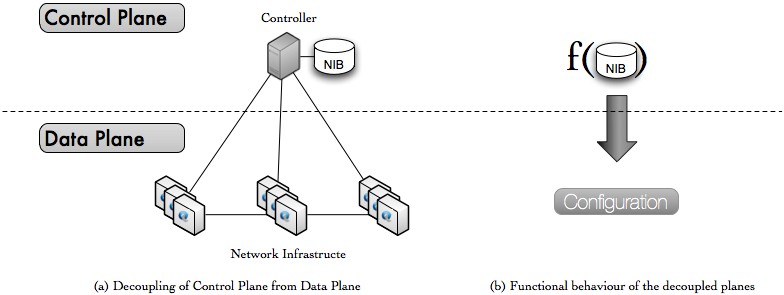
\includegraphics[scale=0.5]{pic/sdn-2d.png}
  \caption[Logical and Physical representation of the SDN architecture]{\textbf{Logical and Physical representation of the SDN architecture}: \textbf{(a)} The controller maintains a connection to the network devices residing in the data plane. The Network Information Base (NIB) contains all the relevant network state (e.g., topology information). \textbf{(b)} The control plane can be represented as a function wich implements the network goals and is dependent of the state stored in the NIB. The result of this function is the configuration of the forwarding state of the data plane.}
  \label{fig:sdn.2d}
\end{figure}

In order to separate the control plane from the data plane it is necessary that the latter implements an interface that allows the configuration of the network devices from the control plane. OpenFlow \cite{openflow} is the most common protocol  that implements this interface and  enables the decoupling of both planes. OpenFlow requires forwarding to be based on flows - a sequence of packets with specified headers in common and allows the control plane to manipulate the flow-based forwarding tables present in network devices. This devices recognize flows (e.g., \emph{any tcp packet destined to port 80} or \emph{any ip packet destined to 1.1.1.1}) and associate them with actions (e.g., \emph{drop packet}, \emph{forward to port $x$}, \emph{forward to controller}). Matching flows have associated actions as opposed to unmatching flows that should be forwarded to the controller. This method has the advantage of possibly redirecting only one packet per flow to the controller (which enables scalability). The SDN architecture also requires the data plane devices to provide the control plane with  updates relevant for the Network Information Base (NIB) such as topology changes  (e.g., \emph{link up}, \emph{link down}).  

The architectural change brought by SDN has the  advantage of
radically changing  the way networking is performed  without changing
the TCP/IP host-to-host stack. The fact that configuration is now
software driven, coupled with the logical centralization of the
network state in the NIB, allows simple and automatic deployment,
configuration and development of  control functionalities. 

 It is worth pointing out that Software Defined Network is not just an
 artifact for the scientific community, but it is also being adopted
 by the industry. For example, Google has deployed a Software Defined
 WAN (Wide Area Network) to connect their datacenters
 \cite{Hoezle:2012uq}. Additionally, this company and other industry
 partners (Yahoo, Microsoft, Facebook, Verizon and Deutsche Telekom,
 Nicira, Juniper, etc.) have formed the Open Network Foundation (ONF)
 \cite{onf} - a non-profit organization  responsible for the
 standardization process of SDN technology. Finally, several network
 hardware vendors currently support OpenFlow \cite{openflow}. Examples
 include IBM, Juniper, and HP. 

\subsection{Distributed Control Plane}
There are several reasons for the distribution of the control plane. In fact, distributed controllers already exist \distcontrollers. We present the following arguments supporting the distribution of the control plane: 

\begin{itemize}
\item[] \textbf{Scalability:}  The controller resources (memory and CPU) do not support all network sizes and dynamics.  Memory contains the network state and the CPU is used for processing network events - mainly new flow events. The use of both these resources grows linearly with the size of the network managed by the control plane eventually leading to  resource exhaustion. Thus, for a scalable control plane it is required to distribute the network state and/or flow processing; 
\item[] \textbf{Performance:}  Scalability may partially be considered for performance reasons also. However, there are more intransigent performance requirements such as latency in Wide Area Networks (WAN's) where big latency penalties may be observed between the  control and data plane  communication; 
\item[] \textbf{Fault Tolerance:} Network control applications built in the controller  may require the availability and durability of the service. Even if failures in the control plane are inevitable, it is desirable to tolerate those without disrupting the  control service. 
\end{itemize}

%TODO - set the number on switches. 
\textbf{Scalability} is a fundamental reason for distributing. Although centralized controllers have been reported  to handle  tens of thousands of hosts \cite{Casado:2007kb}  there are limits in resources that will eventually lead to their exhaustion. These limits are easily reached in current data centers and WANs - in a technical report \cite{Scott:2012tt}, covering fault localization in SDN stacks, we can find referenced numbers of datacenters  that easily reach thousands of switches and hundred of thousands hosts. Additionally in \cite{Tootoonchian:2012uia} references are presented that have found median flow arrival rates of 100K flows per second for a 1500-server cluster as well as spikes of 10M flows arrivals for networks with 100 switches. These numbers strongly  suggest distributing the control plane in order to shield controllers from a large number of network events. 
The \textbf{performance} reason presented may not be the only one, but it is fundamental. At the time of writing only one SDN enabled WAN is known \cite{Hoezle:2012uq}, but given its publicized success one could expect more to follow. Even though the control plane only requires processing  the first packet in flow arrivals, the latency established in this communication must be minimal such that network applications are not noticeable affected. Distribution can mitigate the latency problem by bringing the control plane closer to the data plane (e.g., as done by Kandoo \cite{Yeganeh:2012jm}). 
%TODO - controller placement problem finds that only one controller is enough,  
Finally, \textbf{fault tolerance} is a necessary requirement for several networks applications that require more than \emph{best-effort} delivery of packets. As control plane failures are inevitable, one must guarantee the availability and safety of network control operations. Notice that in centralized control planes the failure of the controller may imply the loss of connectivity through all the network. 

Fundamental principles such as the  Brewer's CAP theorem \cite{Brewer:fk} (formally proven by Gilbert and Lynch \cite{Gilbert:2002il}) are an example of classic distribution tradeoffs. This theorem states that a distributed system may be simultaneously (i.e., at the same time) qualified with only two of the following properties: consistency, availability and partition-tolerance. Furthermore, since supporting partition-tolerance implies tolerating arbitrary message loss  \cite{Gilbert:2002il},  the vast majority of systems are forced to choose between availability and consistency. This choice also applies to the distribution of the control plane. 

The tradeoffs associated with this choice have already been studied by Levin et al. \cite{Levin:2012bt} in the context of SDN. This work found that two control applications (load balancers)  that differ in the choice between availability and consistency have different optimality results. Levin et al. shows also that when availability is chosen the control application optimality\footnote{In the context of the load balancer optimality is equivalent to the most effective use of all paths in the network.} is significantly degraded. In spite of  not all control applications effectively have optimality requirements that are affect by the choice, similar tradeoffs arise in other applications such as: firewalls, intrusion detection and routing. 

As well as degrading optimality, favoring availability also affects transparency - the property of a distributed system to appear as a centralized service to its users. To explain, the choice of availability implies that the user of the system must be aware of the lack of consistency. Thus, if correctness or optimality are relevant for the user, additional effort and reasoning is required in the interaction with the service. 

Currently, often-cited distributed control planes as Onix \cite{Koponen:2010th} or HyperFlow  \cite{Tootoonchian:2010vy} favor availability over consistency. To be true Onix allows the choice to be made between availability and consistency for different control applications. However this choice reveals a less transparent and complex API that forces users to reason about correctness and problems that may arise from the inconsistency of data in the distribution process. Additionally we believe that Onix choices for supporting consistent are not the best\footnote{This argument will be expanded in future versions of this document. For now, it suffices to say that Onix uses transactional databases replicated through the distributed state machine model which result in significant performance limitations \cite{Koponen:2010th}.}.

In our work we favor consistency and consequently transparency in the distribution of the control plane. This is not to say that our system will not show high availability characteristics as much as system favoring availability have inconsistent results. However, there are networks that have control requirements that are best fit with consistency over availability (and vice versa) as discussed by Levin et al. \cite{Levin:2012bt}. 

%In summary, it is usual in distributed systems to choice between consistency and availability. While the latter is informally associated with correctness and latency penalties, the former is associated with incorrectness and scalability. 
 %TODO - can do better. Tradeoffs between scalability, performance and fault tolerance. 
%  Even if \textbf{scalability} is necessary it is not straightforward what is the best way to adopt it. The distribution method choosen must lower the usage of resources and not raise it. For this reason a controller instance must shield event processing from other controllers as well as local state. Equally problematic is the \textbf{performance} issues associated with latency. If we distribute for minimal latency in control to data plane communication we have to minimize the inter-controller communication as it can easily present latency penalties. Finally \textbf{fault tolerance}  presents challenges as it is necessary to perform failure detection and take appropriate measures to take over one controller functions without disrupting the network functional behavior and correctness. The usual solution is to replicate, but this  may affect the scalability of the controller. 

% Other challenges are associated with the distribution of the control plane such as correctness and simplicity of network management applications built on top of it. Consider, as an example, a simple SDN application that contributes to the Network Information Base with high-level namespaces bindings (e.g., user names and associated dynamic IP). Intransigent applications requirements such as logging and access control enforcement then it is strictly necessary to guarantee  that the failure of controllers does not implies the loss of any information currently being tracked. As another example a distributed control plane is more prone to correctness errors as loops or even black holes caused by inconsistency of the network state. Inconsistency, even if  transient, may cause cyclic or conflicting network paths. Notice however, that correctness of applications may always be guaranteed if applications are fully aware of the distribution mechanisms employed by the control plane.\\
%TODO - inconsistent vs consistentcy tradefoof. 
% \subsection{State Machine Replication}
% TO BE WRITTEN: MOTIVATED BY CURRENT PERFORMANCE OF STATE MACHINE REPLICATION. 

\section{Objectives}

%The objective of the experiments covered in this chapter  is to analyze the workloads generated by these applications to thereafter measure the performance of the data store when subject to such realistic demand caused by real applications.

\section{Contributions}
%REFUTABLE CLAIMS WITH FORWARD REFERENCES 
\section{Planning}
\section{Thesis Organization}


This document is structured as following: 
\begin{itemize}
\item Chapter \ref{chapter:1} – AAA 
\item Chapter \ref{chapter:2} – BBB 
\end{itemize}

%%% Local Variables: 
%%% mode: latex
%%% TeX-master: "../PEI"
%%% End: 
